\documentclass{beamer}

\usetheme{Hannover}
\setbeamertemplate{footline}[frame number]

\setbeamertemplate{blocks}[rounded]%
[shadow=false]

\setbeamercolor{block title}{fg=black,bg=blue!20}    
\setbeamercolor{block body}{fg=black,bg=blue!10}      
\setbeamercolor{block body alerted}{fg=white,bg=red}

\definecolor{myblue}{RGB}{1,15,150}

% % definition by cases in equations
% %% The environment cases* handles the second column as text
\usepackage{mathtools}
% Options for hyperref
\hypersetup{
  colorlinks = true,
  linkcolor = myblue,
  urlcolor = magenta
}

\title{The STOC free model}
\subtitle{Objectives, hypotheses and model overview}
\author[Madouasse \textit{et al.}]{Aurélien Madouasse \texorpdfstring{\\}{}\& \texorpdfstring{\\}{}the STOC free consortium}
\institute{\url{https://www.stocfree.eu/}}

%\titlegraphic{
\includegraphics[width=\textwidth]{imgs/title_page_bg.png}}


\begin{document}
{
%  \usebackgroundtemplate{
\includegraphics[width=\paperwidth]{imgs/title_page_bg1.png}}%
  \usebackgroundtemplate{
\includegraphics[width=1.1\paperwidth]{imgs/title_page_bg1.png}}%
  \maketitle
}

\begin{frame}
\frametitle{Table of Contents}
  \tableofcontents
\end{frame}  

\section{Context and objectives}

\begin{frame}
\frametitle{Table of Contents}
  \tableofcontents[currentsection]
\end{frame}  


\begin{frame}
\frametitle{Infectious diseases of cattle}
\framesubtitle{Regulated diseases}
\begin{itemize}
  \item{Public health threats}
  \item[]{\scriptsize e.g. Tuberculosis}
  \item{Economic impact}
  \item[]{\scriptsize e.g. Foot and mouth disease}
  \item{Legislation on how to perform surveillance in order to substantiate freedom from disease}
  \item{Every country performs surveillance in the same way $\rightarrow$ comparable output}
  \item[$\Rightarrow$]{\textcolor{red}{\textbf{Input-based surveillance}}}
 \end{itemize}
\end{frame}

\begin{frame}
\frametitle{Infectious diseases of cattle}
\framesubtitle{Non-regulated diseases}
 \begin{itemize}
  \item{A lot of important infectious diseases are not regulated but have regional / national control programmes in place}
  \item[]{\scriptsize e.g. BVD, paratuberculosis $\ldots$}
  \begin{itemize}
   \item{No \emph{legal} prescription on the way to perform surveillance}
   \item{Important diversity in the design of surveillance programmes}
   \item{The \emph{free status} in one programme can have a different meaning than the \emph{free status} in another programme}
  \end{itemize}
  \item[$\Rightarrow$]{Creates difficulties when trading animals between herds enrolled in different programmes}
  \item[$\Rightarrow$]{\textcolor{red}{\textbf{Output-based surveillance}}: production of an output that is comparable regardless of the input surveillance data}
    \end{itemize}
\end{frame}

\begin{frame}
\frametitle{A method for output-based surveillance}
\begin{itemize}
\item{Need for a method taking inputs from diverse surveillance programmes able to produce an output that is comparable}
  \begin{itemize}
   \item{Structure of the method/model determined by what is common across surveillance programmes}
   \item{Probability of freedom from infection estimated in a given programme from:}
   \begin{itemize}
    \item{surveillance data available in the programme}
    \item{relevant knowledge (e.g. test characteristics)}
   \end{itemize}
  \end{itemize}
\end{itemize}
\end{frame}

\begin{frame}
\frametitle{Control programmes}
\framesubtitle{Common features}
\begin{itemize}
 \item{\emph{Control} programmes against cattle non-regulated diseases: prevalence $>0$}
 \item{Objective: disease control or eradication}
 \item{Organised at regional or country level}
 \item{Rely on a surveillance component for the identification of infected herds or animals}
 \item{Detection of infection followed by control phase}
 \item{Surveillance performed in all participating herds}
 \item{Herd tested repeatedly over time}
  \begin{itemize}
   \item[$\Rightarrow$]{Longitudinal data}
  \end{itemize}
\end{itemize}
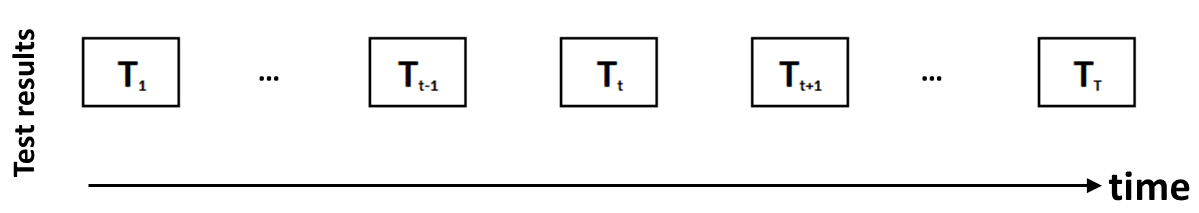
\includegraphics[width=\textwidth]{imgs/longitudinal_data.png}
\end{frame}

\begin{frame}
\frametitle{Control programmes}
\framesubtitle{Common features}
\begin{itemize}
 \item{Tests are imperfect}
 \begin{itemize}
  \item{Sensitivity: $Se = p(T^+|D^+) < 1$}
  \item{Specificity: $Sp = p(T^-|D^-) < 1$}
 \end{itemize}
 \item[$\Rightarrow$]{Uncertainty in the true status of tested animals / herds}
\end{itemize}
\center
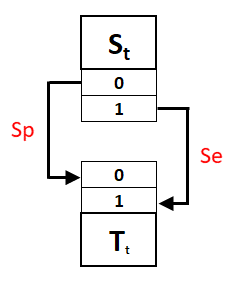
\includegraphics[width=.3\textwidth]{imgs/SeSp.png}
\end{frame}


\section{Modelling framework}
\begin{frame}
\frametitle{Table of Contents}
  \tableofcontents[currentsection]
\end{frame} 

\begin{frame}
\frametitle{Modelling objectives}
\begin{itemize}
 \item{Objective: Predict herd level probabilities of \emph{(freedom from)} infection from longitudinal test data collected as part of surveillance programmes against endemic infectious diseases of cattle}
 \item{The modelling framework should:}
 \begin{itemize}
  \item{Allow the use of longitudinal data i.e. account for the fact that sequences of test results are not random}
  \item{Account for imperfect test information}
 \end{itemize}
\end{itemize}
\end{frame}

\begin{frame}
\frametitle{Hidden Markov models}
\begin{itemize}
 \item{Hidden Markov Models (\textbf{HMM}s) model a latent discrete variable with a Markovian dynamics, whose state at a given time determines the distribution of an observed variable}
  \begin{itemize}
   \item{\textbf{discrete variable}: the variable of interest can be in 1 of $k$ states. In the STOC free model, $k=2$ (positive or negative status)}
   \item{\textbf{latent variable}: this discrete variable is not directly observed. In the STOC free model, the \textbf{latent status} determines the probability of a negative or positive test result through test sensitivity and specificity}
   \item{\textbf{Markovian dynamics}: the latent status is modelled in discrete time steps. The latent status at time $t$ only depends on the status at time $t-1$. The probabilities of transition between the $k$ states between 2 time points are described by a $k$ x $k$ transition matrix.}
  \end{itemize}
\end{itemize}
\end{frame}

\begin{frame}
\frametitle{Representation of surveillance programmes as HMMs}
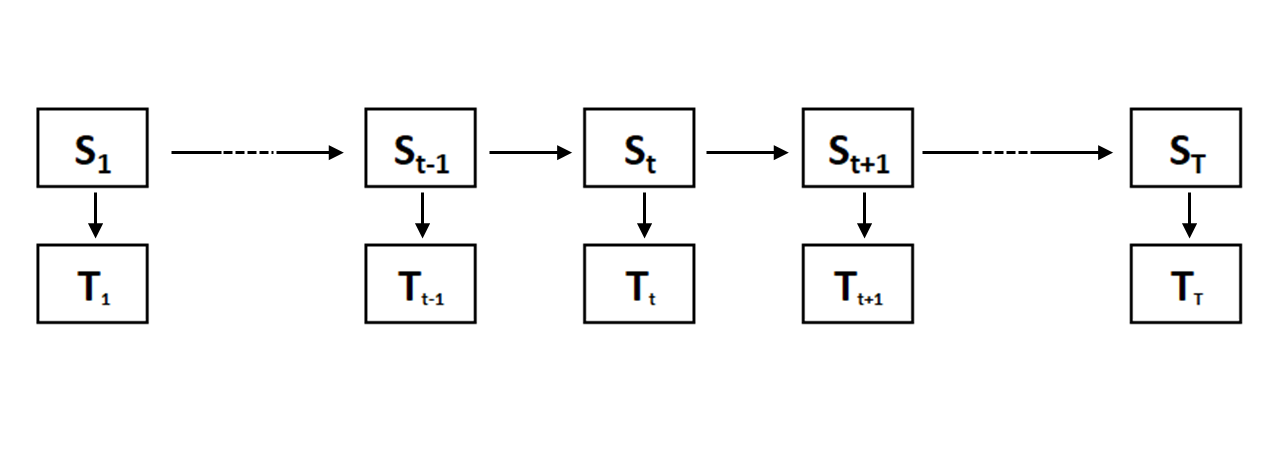
\includegraphics[width = \textwidth]{imgs/surveillance_programmes_HMMs.png}
\begin{itemize}
 \item{$S_t$: latent status of interest at time $t$ , from $t=1$ to $t=T$}
 \item{$T_t$: test result at time $t$}
\end{itemize}
\end{frame}

\begin{frame}
\frametitle{Representation of surveillance programmes as HMMs}
\framesubtitle{Status dynamics}
\begin{columns}
\begin{column}{0.6\textwidth}
\begin{itemize}
  \item{Time steps of equal duration}
  \begin{itemize}
   \item[]{\scriptsize(Discrete-time model)}
  \end{itemize}
  \item{Herd status at time $t$ depends on herd status at time $t_1$}
  \begin{itemize}
   \item[]{\scriptsize(Markovian property)}
  \end{itemize}
\end{itemize}
\vspace{.5cm}
$$S_t \sim Bernoulli(\pi_t)$$
$$\pi_t = \begin{cases*} \tau_1 &if $S_{t-1}=0$ \\
                        \tau_2 &if $S_{t-1}=1$ \end{cases*}$$
\end{column}
\begin{column}{0.4\textwidth}
\vspace{2cm}
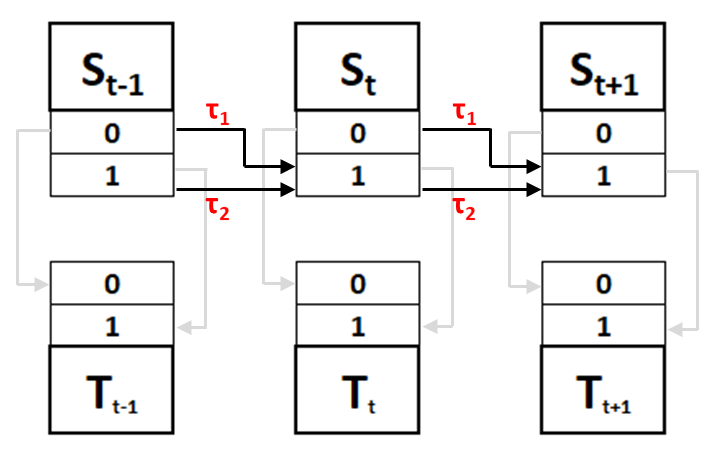
\includegraphics[width = 1.1\textwidth]{imgs/dynamics.png}
\end{column}
\end{columns}
\end{frame}

\begin{frame}
\frametitle{Representation of surveillance programmes as HMMs}
\framesubtitle{Status dynamics}
\begin{columns}
\begin{column}{0.6\textwidth}
\begin{itemize}
  \item{Herd level probability of new infection ($\tau_{1t}$) modelled as a function of one or several risk factors ($X_t$) using logistic regression}
\end{itemize}
\vspace{.5cm}
$$ln(\frac{\tau_{1t}}{1 - \tau_{1t}}) = X_{t} \theta$$
\end{column}
\begin{column}{0.4\textwidth}
\vspace{2cm}
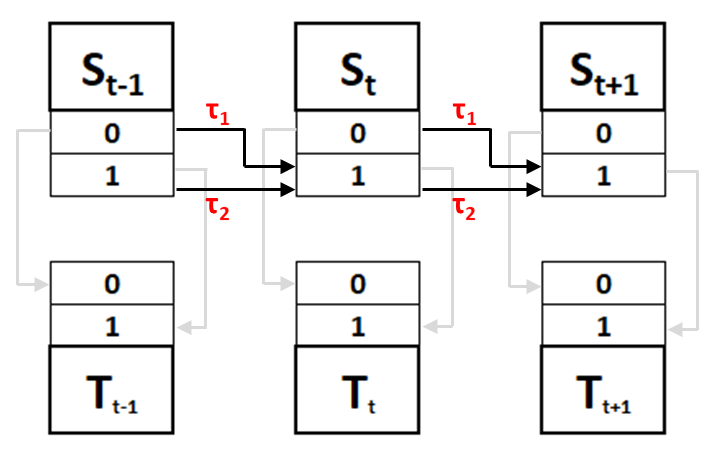
\includegraphics[width = 1.1\textwidth]{imgs/dynamics.png}
\end{column}
\end{columns}
\end{frame}

\begin{frame}
\frametitle{Representation of surveillance programmes as HMMs}
\framesubtitle{Status dynamics}
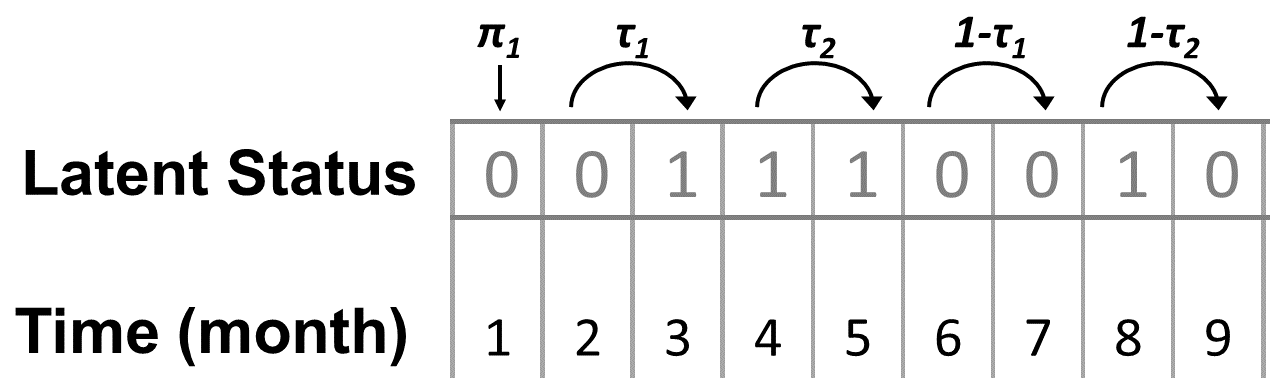
\includegraphics[width = \textwidth]{imgs/infection_dynamics.png}
\end{frame}

\begin{frame}
\frametitle{Representation of surveillance programmes as HMMs}
\framesubtitle{Test results}
\begin{columns}
\begin{column}{0.85\textwidth}
\begin{itemize}
  \item{Herd status at time t is either negative (0) OR positive (1)}
\vspace{2cm}
  \item{Test result at time t is either negative (0) OR positive (1)}
\end{itemize}
\end{column}
\begin{column}{0.15\textwidth}
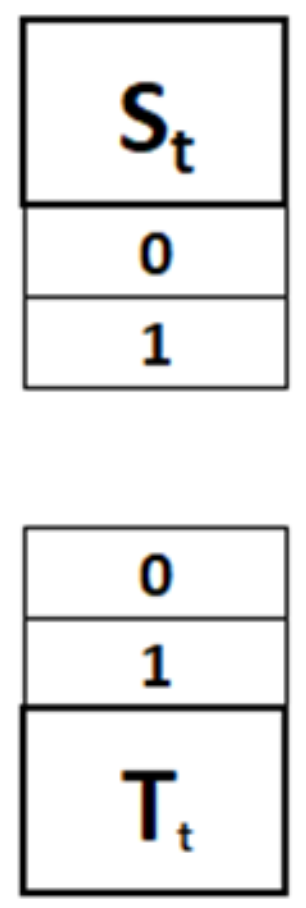
\includegraphics[width = 1\textwidth]{imgs/status_test.png}
\end{column}
\end{columns}
\end{frame}

\begin{frame}
\frametitle{Representation of surveillance programmes as HMMs}
\framesubtitle{Test results}
\begin{columns}
\begin{column}{0.6\textwidth}
\begin{itemize}
  \item{Test results at the herd level}
  \item{Test results depend on the latent status through sensitivity and specificity}
\end{itemize}
\vspace{.5cm}
$$p(T_t = 1) = \begin{cases*} 1 - Sp &if $S_{t}=0$ \\
                              Se &if $S_{t}=1$ \end{cases*}$$
\end{column}
\begin{column}{0.4\textwidth}
\vspace{2cm}
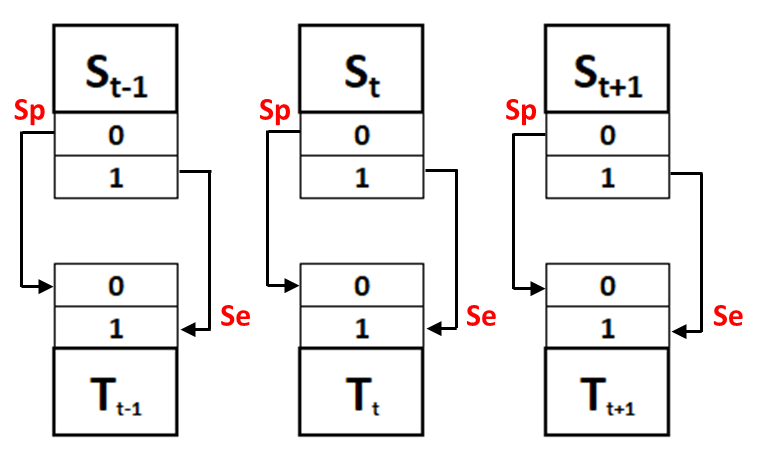
\includegraphics[width = 1.1\textwidth]{imgs/status_test1.png}
\end{column}
\end{columns}
\end{frame}

\begin{frame}
\frametitle{Representation of surveillance programmes as HMMs}
\framesubtitle{Test results}
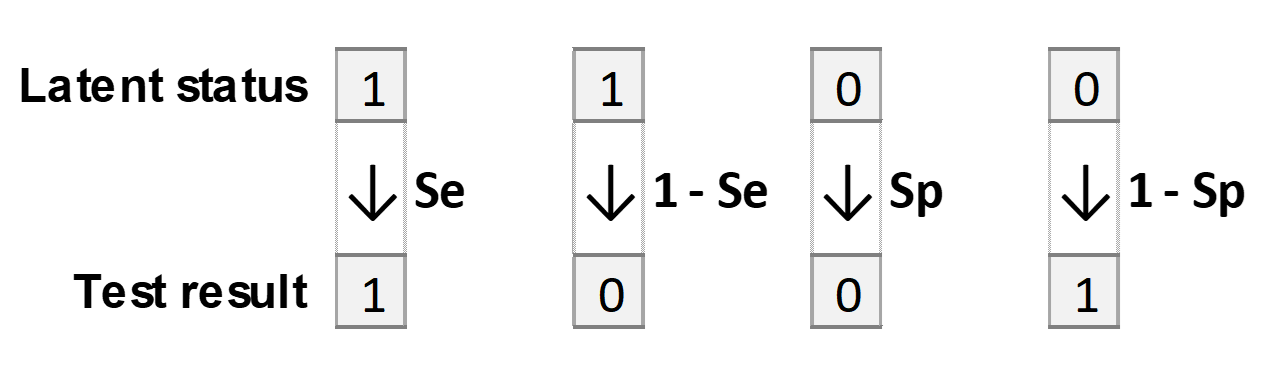
\includegraphics[width = \textwidth]{imgs/test_imperfection.png}
\end{frame}

\begin{frame}
\frametitle{Predictions}

\begin{itemize}
 \item{The model predicts a herd level probability of being status positive at time $T$}
 \item{All the data available up to $T$ are used for parameter estimation}
\end{itemize}
\vspace{.5cm}
\center
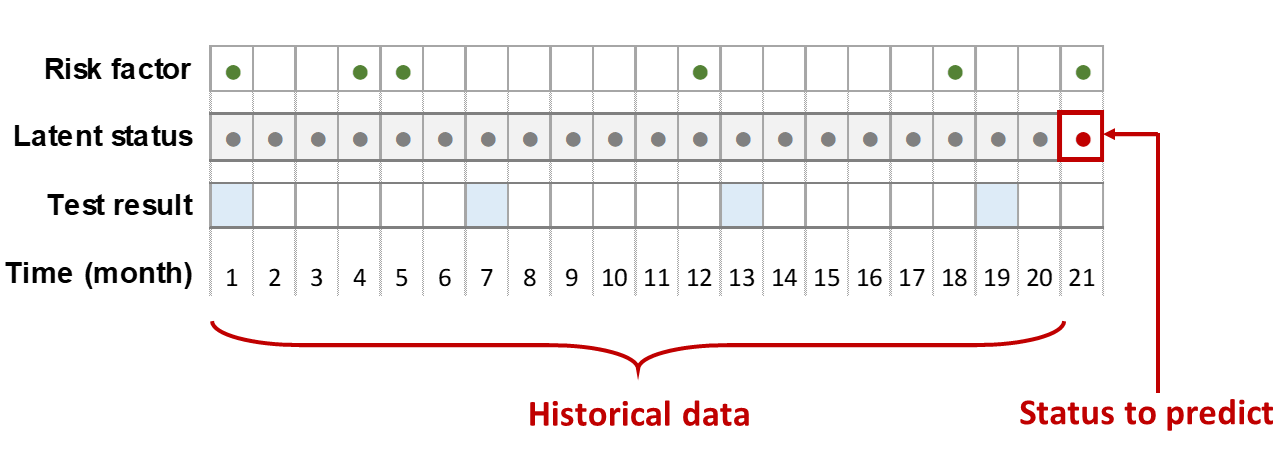
\includegraphics[width = \textwidth]{imgs/modelling_framework.png}
\end{frame}

\begin{frame}
\frametitle{Summary of the different model parameters}
\begin{itemize}
 \item{$\pi_1$: probability of being status positive on the first test month}
 \item{$\tau_1$: probability of becmoing status positive between 2 months}
 \item{$\theta_1, \theta_2 \ldots$: coefficients of the logistic regression for the probability of becoming status positive}
 \item{$\tau_2$: probability of remaining status positive between 2 months}
 \item{$Se$: herd-level test sensitivity}
 \item{$Sp$: herd-level test specificity}
\end{itemize}
\end{frame}

\begin{frame}
\frametitle{The complete model - no risk factor}
$$S_1 \sim Bernoulli(\pi_1)$$
$$S_t \sim Bernoulli(\pi_t) \hspace{.25cm} \forall t > 1$$
$$\pi_t = \begin{cases*} \tau_1 &if $S_{t-1}=0$ \\
                        \tau_2 &if $S_{t-1}=1$ \end{cases*}$$
$$T_t \sim Bernoulli(p(T_t))$$
$$p(T_t) = \begin{cases*} 1 - Sp &if $S_t = 0$ \\
                         Se &if $S_t = 1$ \end{cases*}$$
\end{frame}

\begin{frame}
\frametitle{The complete model - with risk factors}

$$S_1 \sim Bernoulli(\pi_1)$$
$$S_t \sim Bernoulli(\pi_t) \hspace{.25cm} \forall t > 1$$
$$\pi_t = \begin{cases*} \tau_{1t} &if $S_{t-1}=0$ \\ 
                        \tau_2 &if $S_{t-1}=1$ \end{cases*}$$
$$ln(\frac{\tau_{1t}}{1- \tau_{1t}}) = X_{ht} \theta$$                   
$$T_t \sim Bernoulli(p(T_t))$$
$$p(T_t) = \begin{cases*} 1 - Sp &if $S_t = 0$ \\
                         Se &if $S_t = 1$ \end{cases*}$$
\end{frame}


\section{Implementation}

\begin{frame}
\frametitle{Table of Contents}
  \tableofcontents[currentsection]
\end{frame} 

\subsection{Overview}

\begin{frame}
\frametitle{Model implementation}
\begin{itemize}
 \item{Parameter estimation and prediction carried out in a Bayesian framework}
\begin{itemize}
 \item{The framework permits the incorporation of available knowledge using prior distributions}
 \item{Two different programmes can be used to run the model: \href{https://sourceforge.net/projects/mcmc-jags/files/}{JAGS} or \href{https://mc-stan.org}{Stan}}
 \end{itemize}
\end{itemize}
\end{frame}


\subsection{\texttt{STOCfree} package}

\begin{frame}
\frametitle{The \texttt{STOCfree} R package}
\framesubtitle{What is an R package?}
\begin{itemize}
\item[]{
\includegraphics[width=.07\textwidth]{imgs/Rlogo.png}}
\begin{itemize}
 \item{Programming environment for data manipulation and analysis}
 \item{Widely used}
 \item{Free}
\end{itemize}
\item[]{
\includegraphics[width=.07\textwidth]{imgs/Rlogo.png} package}
 \begin{itemize}
  \item{Set of functions gathered to perform specific tasks}
  \item{Users install a package and can use the functions they contain}
  \item{Packages are installed from the web (CRAN, GitHub…)}
 \end{itemize}
\end{itemize}
\end{frame}

\begin{frame}
\frametitle{The \texttt{STOCfree} R package}
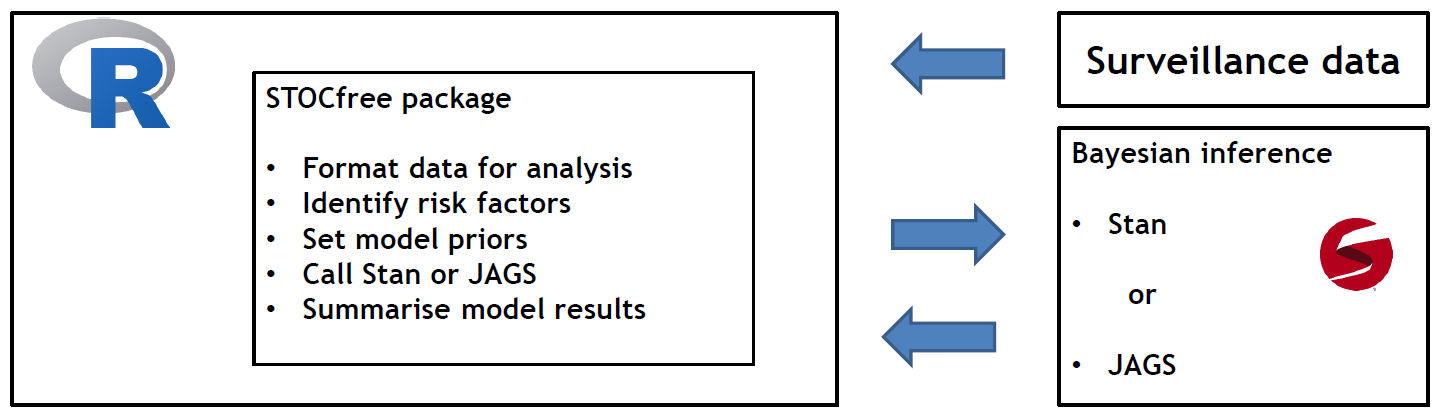
\includegraphics[width=\textwidth]{imgs/STOCfree_package.png}
\end{frame}

\begin{frame}
\frametitle{The \texttt{STOCfree} R package on Github}
\begin{itemize}
 \item{The package is hosted on Github}
 \url{https://github.com/AurMad/STOCfree}
 \item{Github is a server hosting:}
 \begin{itemize}
  \item{The package code}
  \item{The package documentation}
  \item{The history of development and different package versions, using the Git versioning programme}
 \end{itemize}
\end{itemize}
\end{frame}

\begin{frame}
\frametitle{The STOCfree R package on Github}
\begin{itemize}
 \item{All the code is in the \texttt{R} folder}
\end{itemize}
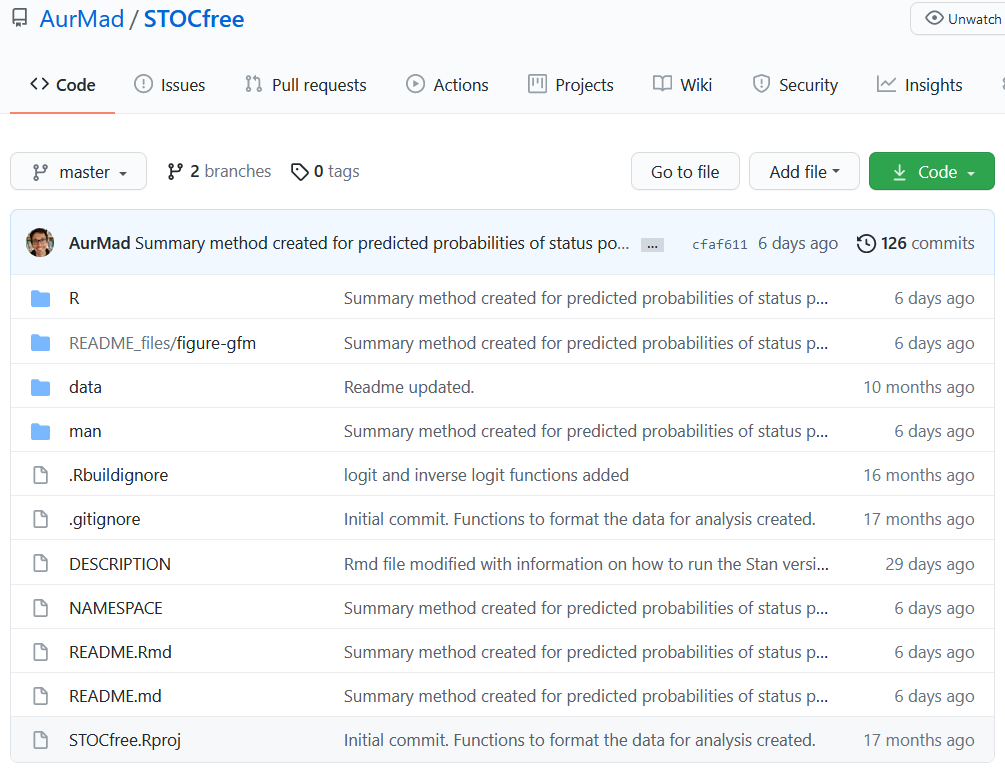
\includegraphics[width=.9\textwidth]{imgs/STOCfree_Github.png}
\end{frame}

\begin{frame}
\frametitle{The STOCfree R package on Github}
\begin{itemize}
 \item{The documentation is at the bottom of the page}
\end{itemize}
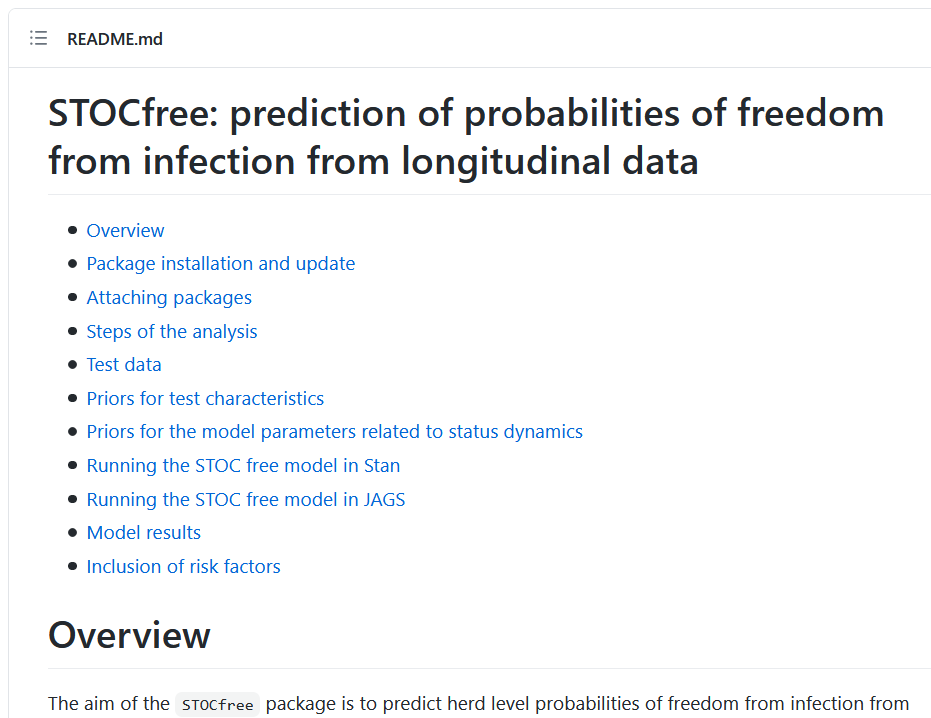
\includegraphics[width=.9\textwidth]{imgs/STOCfree_Github_1.png}
\end{frame}


\section[Application]{Application to the surveillance of BVDV infection in Loire-Atlantique (France)}

\begin{frame}
\frametitle{Table of Contents}
  \tableofcontents[currentsection]
\end{frame} 

\subsection{Data}

\begin{frame}
\frametitle{Data}
\begin{itemize}
 \item{Surveillance data collected as part of a dairy cattle BVD control programme in Loire-Atlantique (France)}
 \begin{itemize}
  \item{All herds tested every 6 months}
  \item{Antibody ELISA on bulk tank milk}
  \item{Data from 1 687 herds between 2014 and 2017}
 \end{itemize}
\end{itemize}
\end{frame}

\begin{frame}
\frametitle{Data}
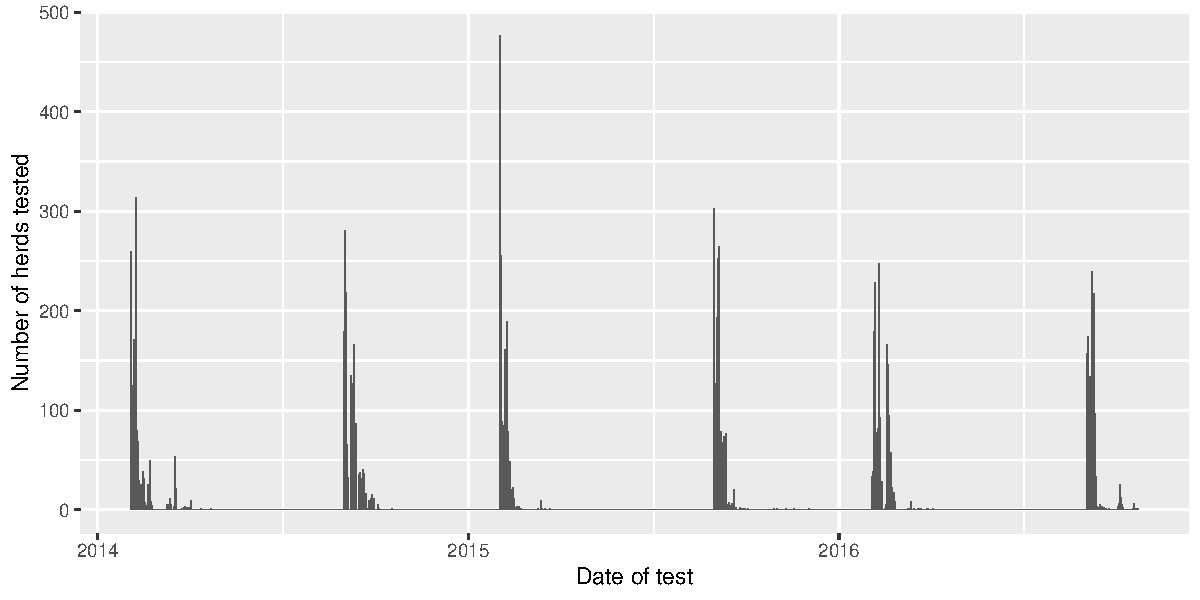
\includegraphics[width=\textwidth]{imgs/distribution_of_test_dates.pdf}
\end{frame}

\subsection{Modelling}

\begin{frame}
\frametitle{Models}
\begin{itemize}
 \item{Four different models incorporating different hypotheses were run in both Stan and JAGS and the results compared}
 \begin{itemize}
  \item{\textbf{Model 1:} Perfect test, no risk factors}
  \item{\textbf{Model 2:} Imperfect test, no risk factors}
  \item{\textbf{Model 3:} Perfect test, risk factors}
  \item{\textbf{Model 4:} Imperfect test, risk factors}
 \end{itemize}
 \item<2->{Risk factors}
 \begin{itemize}
  \item{Two considered: number of cattle introduced, local seroprevalence}
  \item{Only number of cattle introduced retained in the final model}
 \end{itemize}
\end{itemize}
\end{frame}

\begin{frame}
\frametitle{Prior distributions}
\framesubtitle{Perfect test}
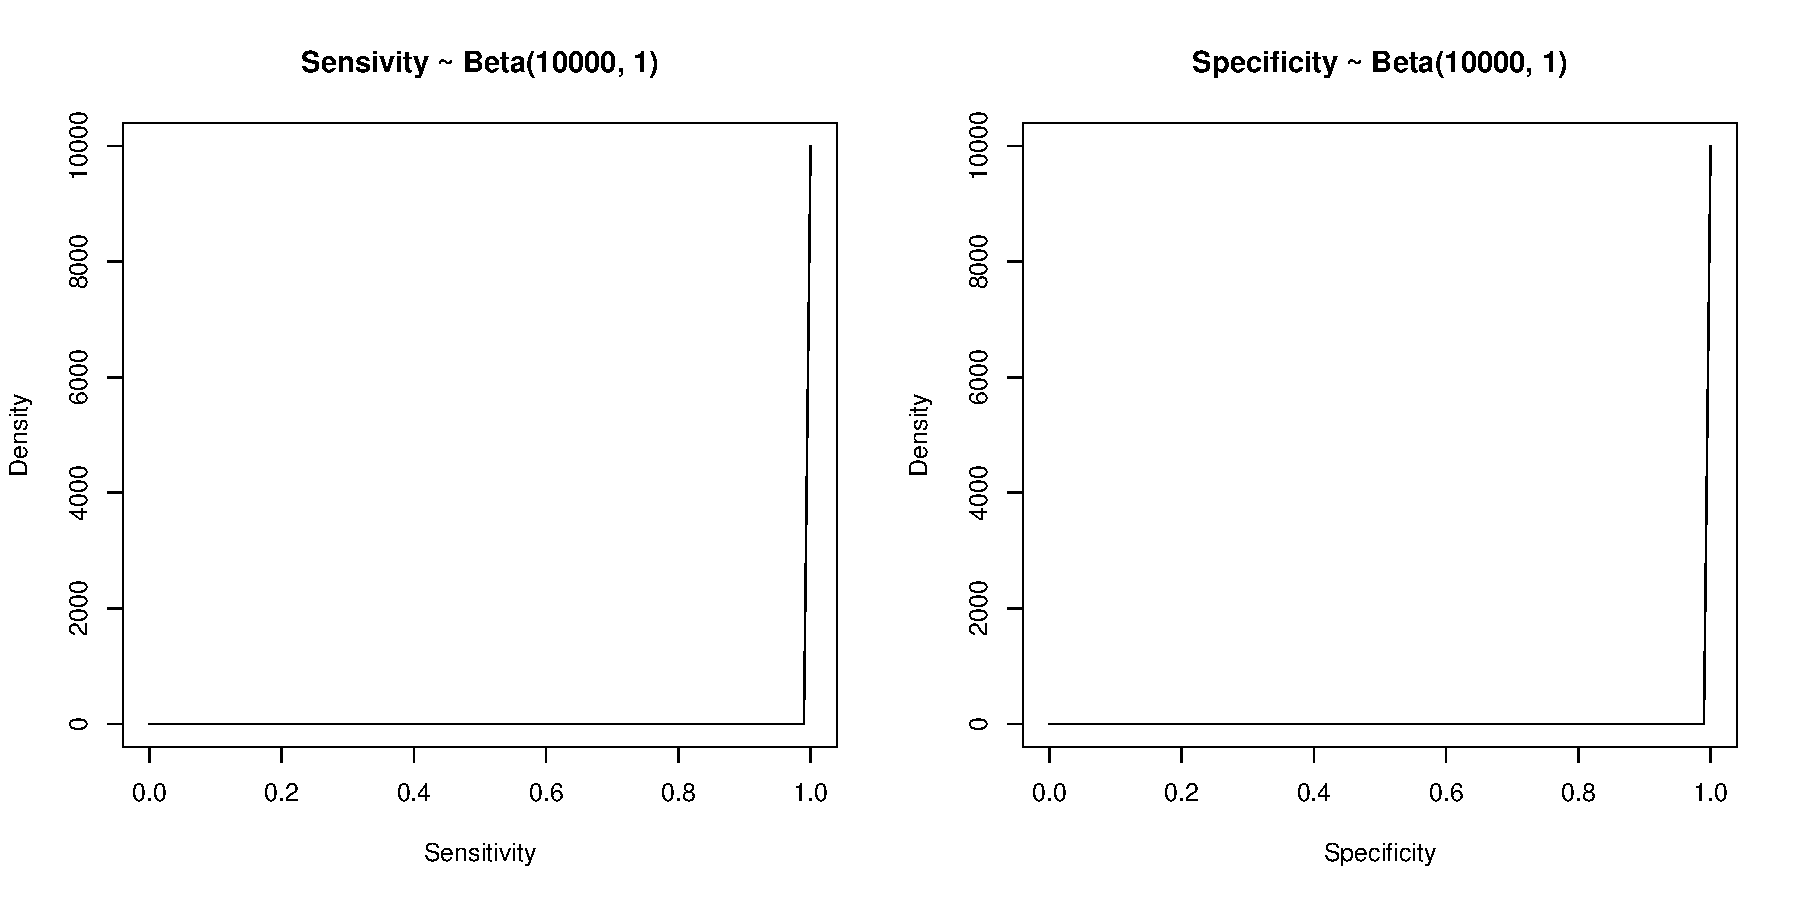
\includegraphics[width=\textwidth]{imgs/priors_perfect_test.pdf}
\end{frame}

\begin{frame}
\frametitle{Prior distributions}
\framesubtitle{Imperfect test}
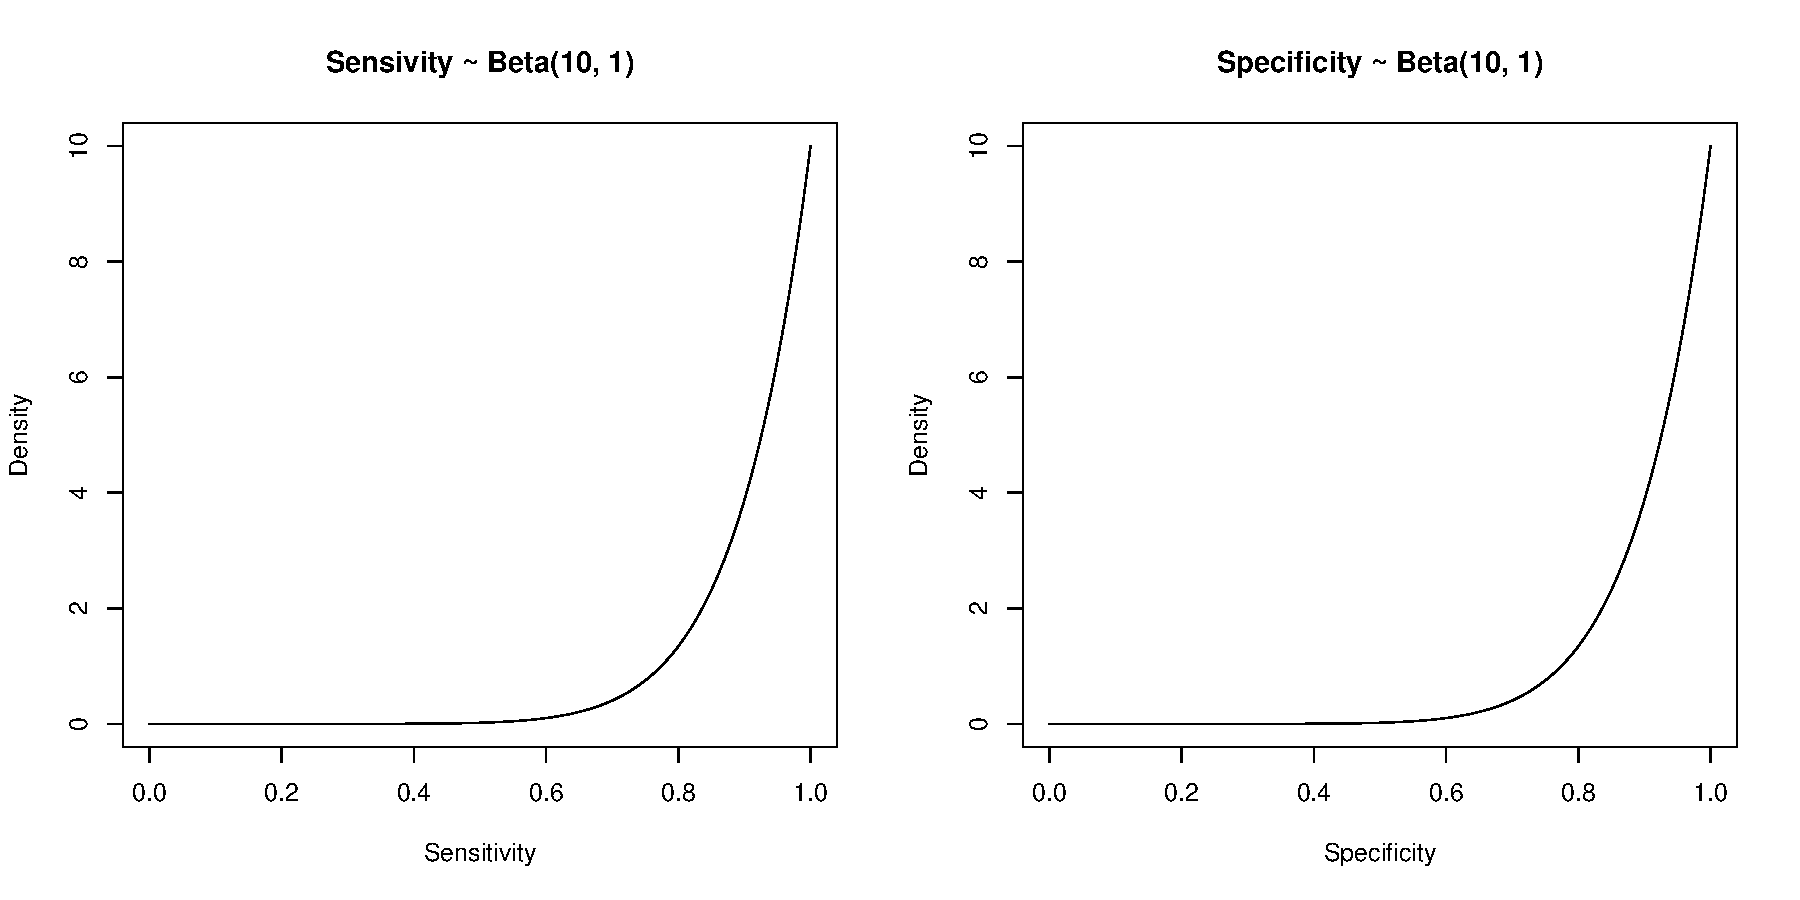
\includegraphics[width=\textwidth]{imgs/priors_imperfect_test.pdf}
\end{frame}

\begin{frame}
\frametitle{Prior distributions}
\framesubtitle{Risk factors: intercept and coefficient}
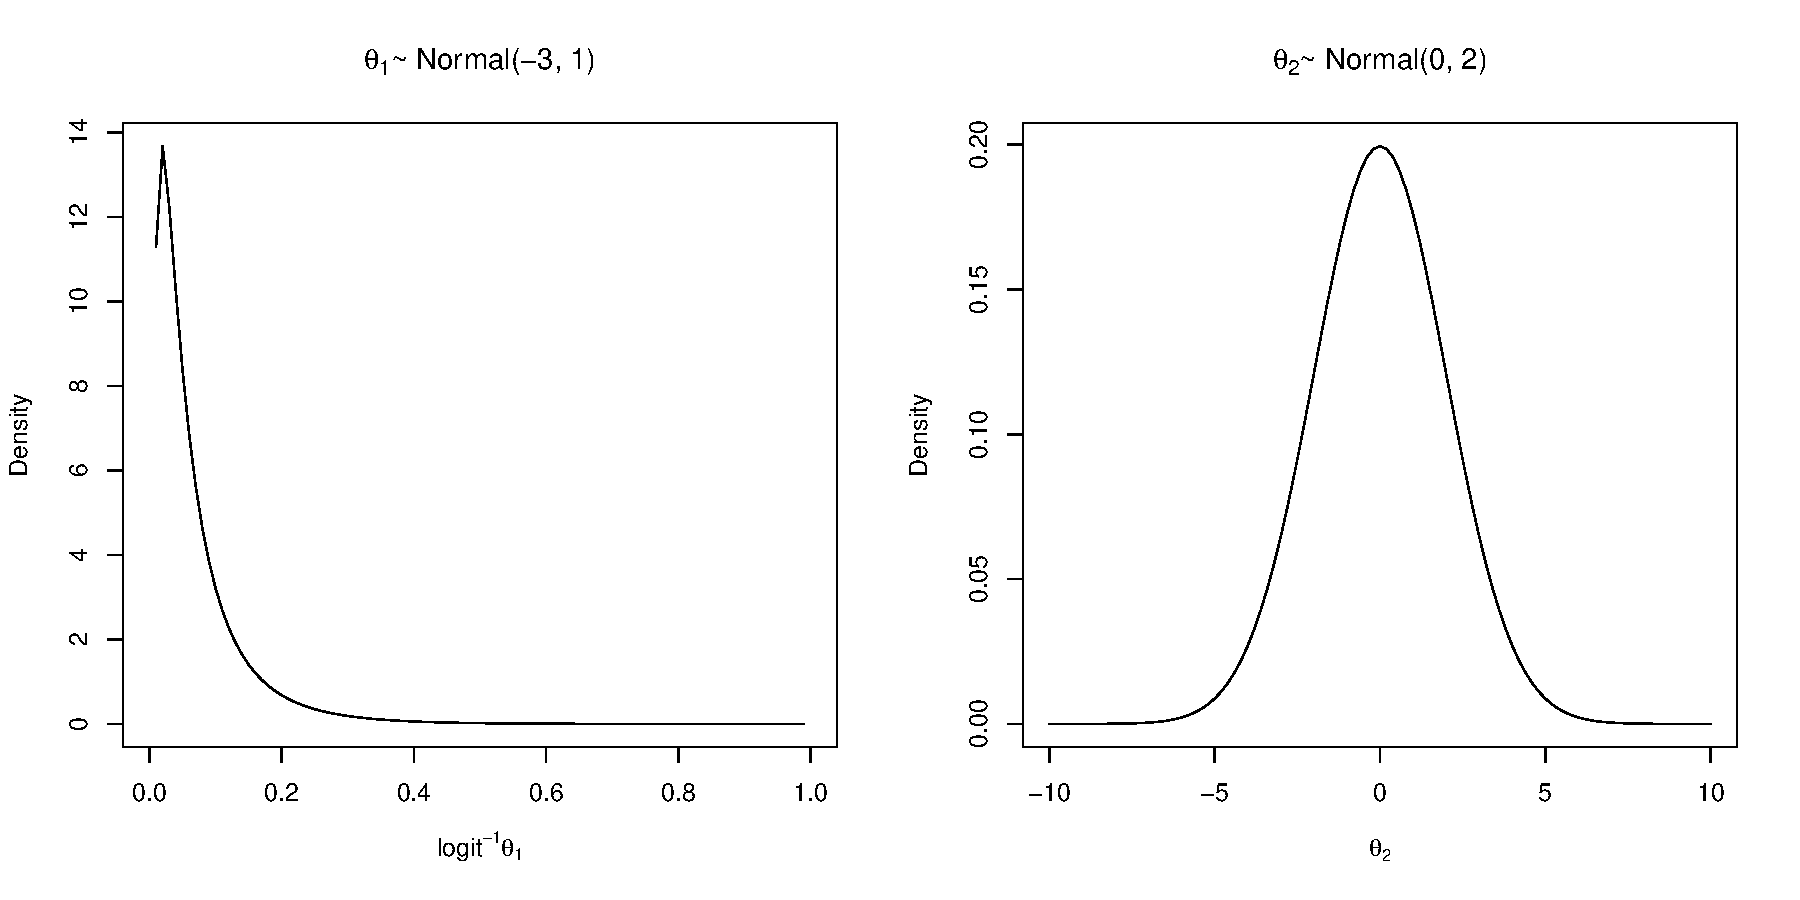
\includegraphics[width=\textwidth]{imgs/priors_thetas.pdf}
\end{frame}

\subsection{Results}

\begin{frame}
\frametitle{Model convergence}
\begin{itemize}
 \item{Convergence much better with the Stan version of the model, especially with imperfect test}
\end{itemize}
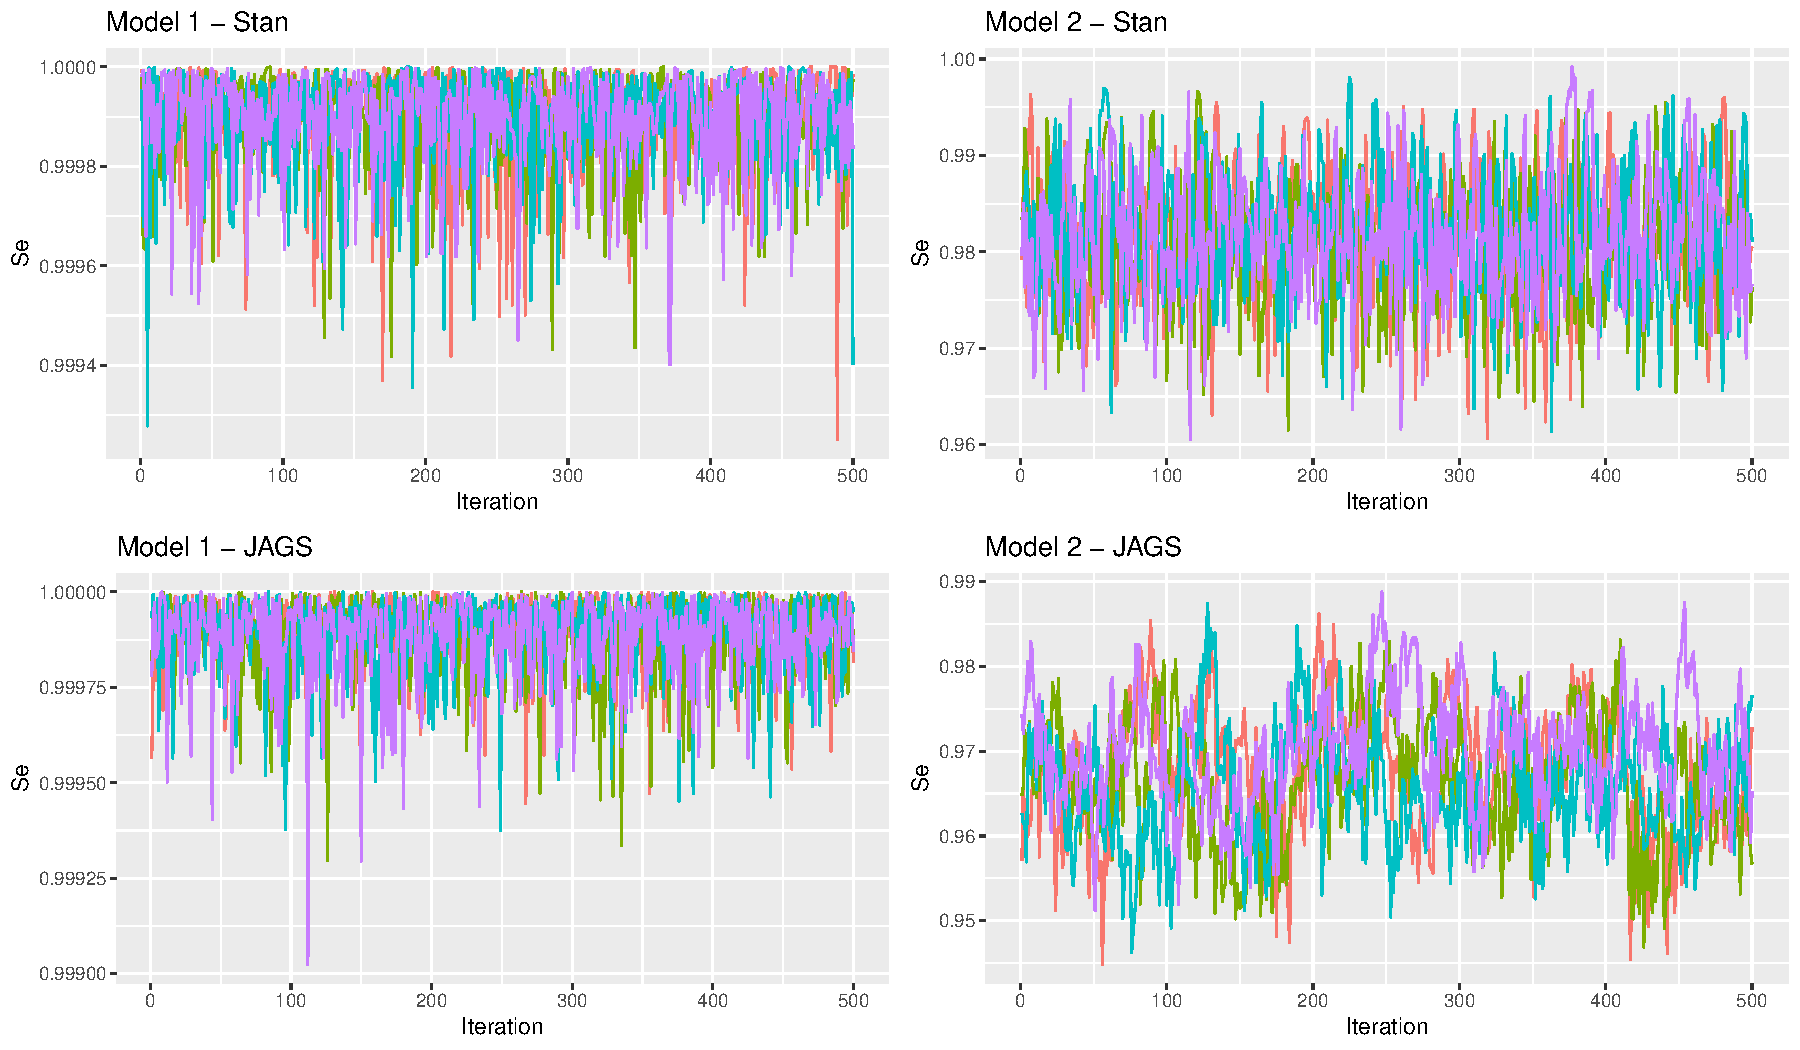
\includegraphics[width=\textwidth]{imgs/traceplots.pdf}
\end{frame}

\begin{frame}
\frametitle{Parameter estimates}
\framesubtitle{Test characteristics}
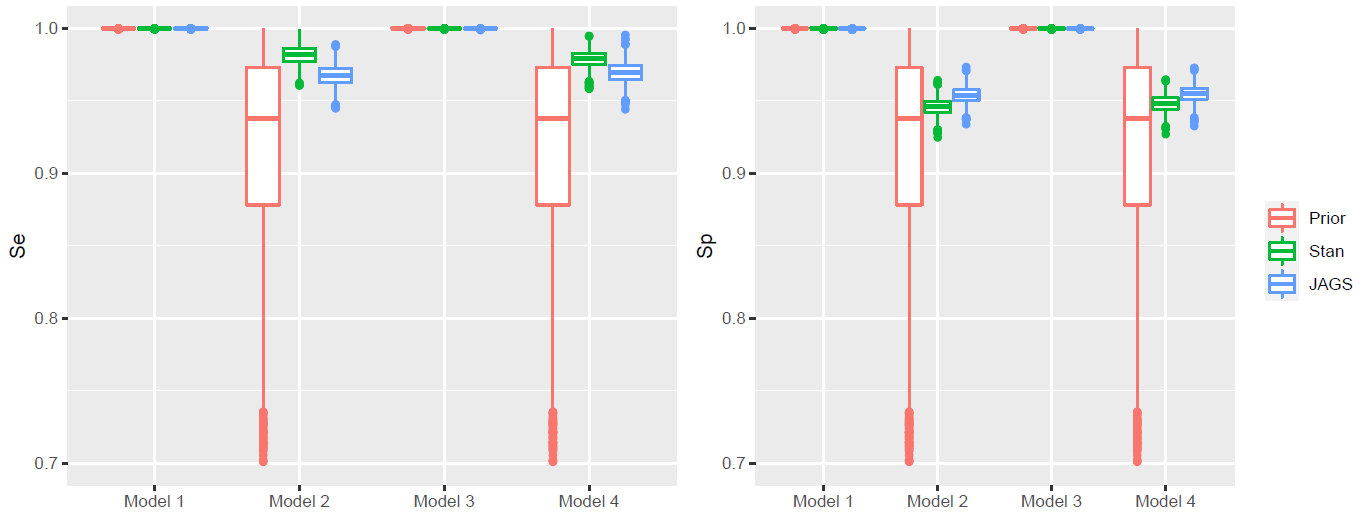
\includegraphics[width=\textwidth]{imgs/model_densities_1.png}
\end{frame}

\begin{frame}
\frametitle{Parameter estimates}
\framesubtitle{Infection dynamics}
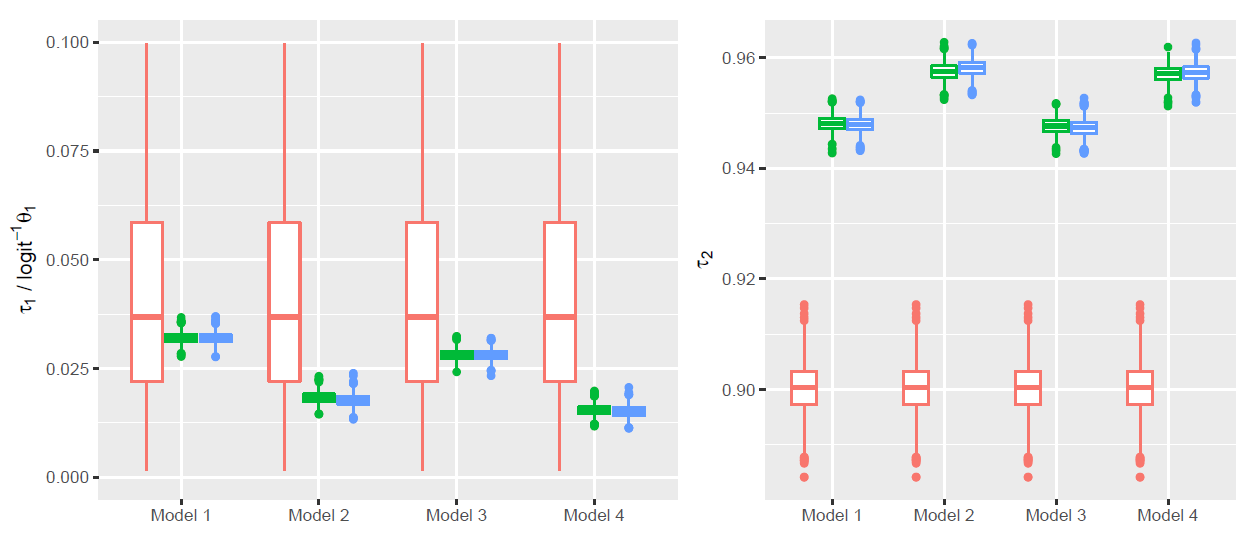
\includegraphics[width=\textwidth]{imgs/model_densities_2.png}
\end{frame}

\begin{frame}
\frametitle{Parameter estimates}
\framesubtitle{Risk factors of new infection}
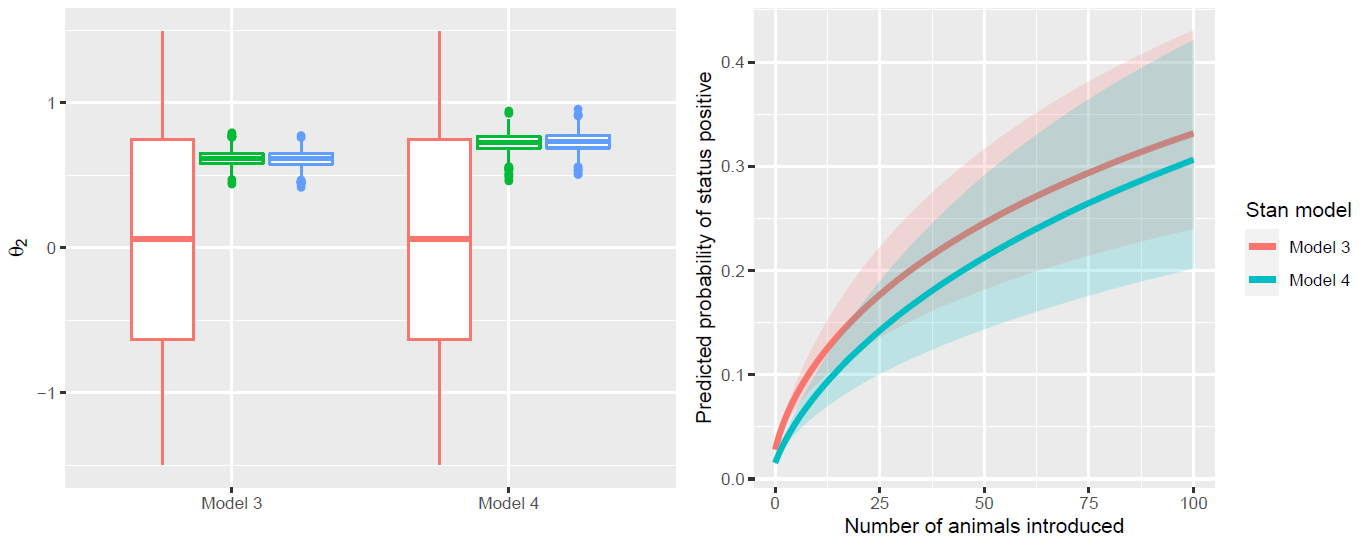
\includegraphics[width=\textwidth]{imgs/model_densities_3.png}
\end{frame}

\begin{frame}
\frametitle{Parameter estimates}
\begin{itemize}
\item{Estimates consistent between JAGS and Stan}
\item{Posterior distributions much narrower and sometimes far from the prior distributions}
\item{The number of cattle introduced increases the probability of infection $\Rightarrow$ increase in the sensitivity of detection}
\end{itemize}
\end{frame}

\begin{frame}
\frametitle{Predicted probabilities of infection}
\begin{itemize}
 \item{Predicted for:}
 \begin{itemize}
 \item{all herds}
 \item{the last month in which a test result was available (October 2016)}
 \end{itemize}
\end{itemize}
\end{frame}

\begin{frame}
\frametitle{Predicted probabilities of infection}
\framesubtitle{Overall posterior distributions}
\centering
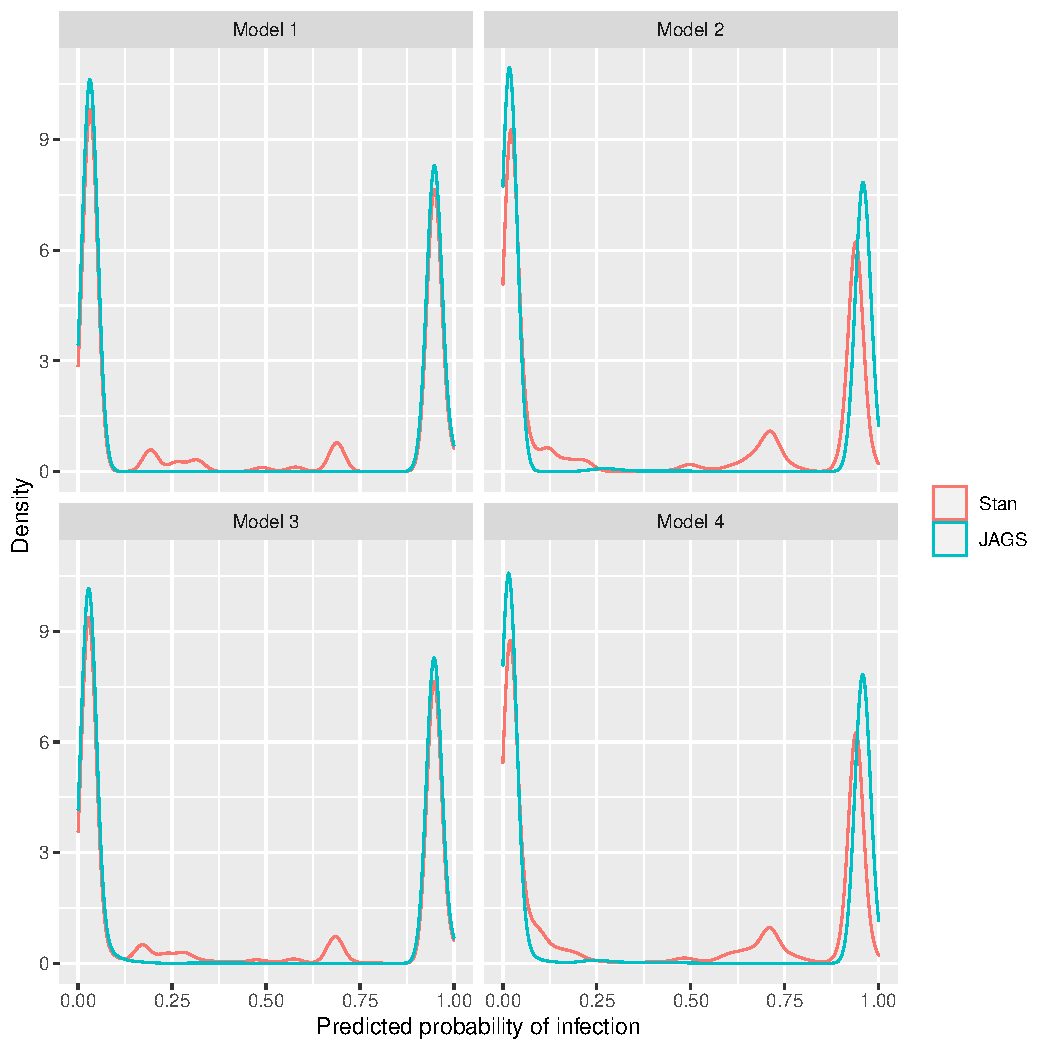
\includegraphics[width=.72\textwidth]{imgs/plot_predicted_proba_all_herds.pdf}
\end{frame}

\begin{frame}
\frametitle{Predicted probabilities of infection}
\framesubtitle{Posterior distributions for 4 herds}
\centering
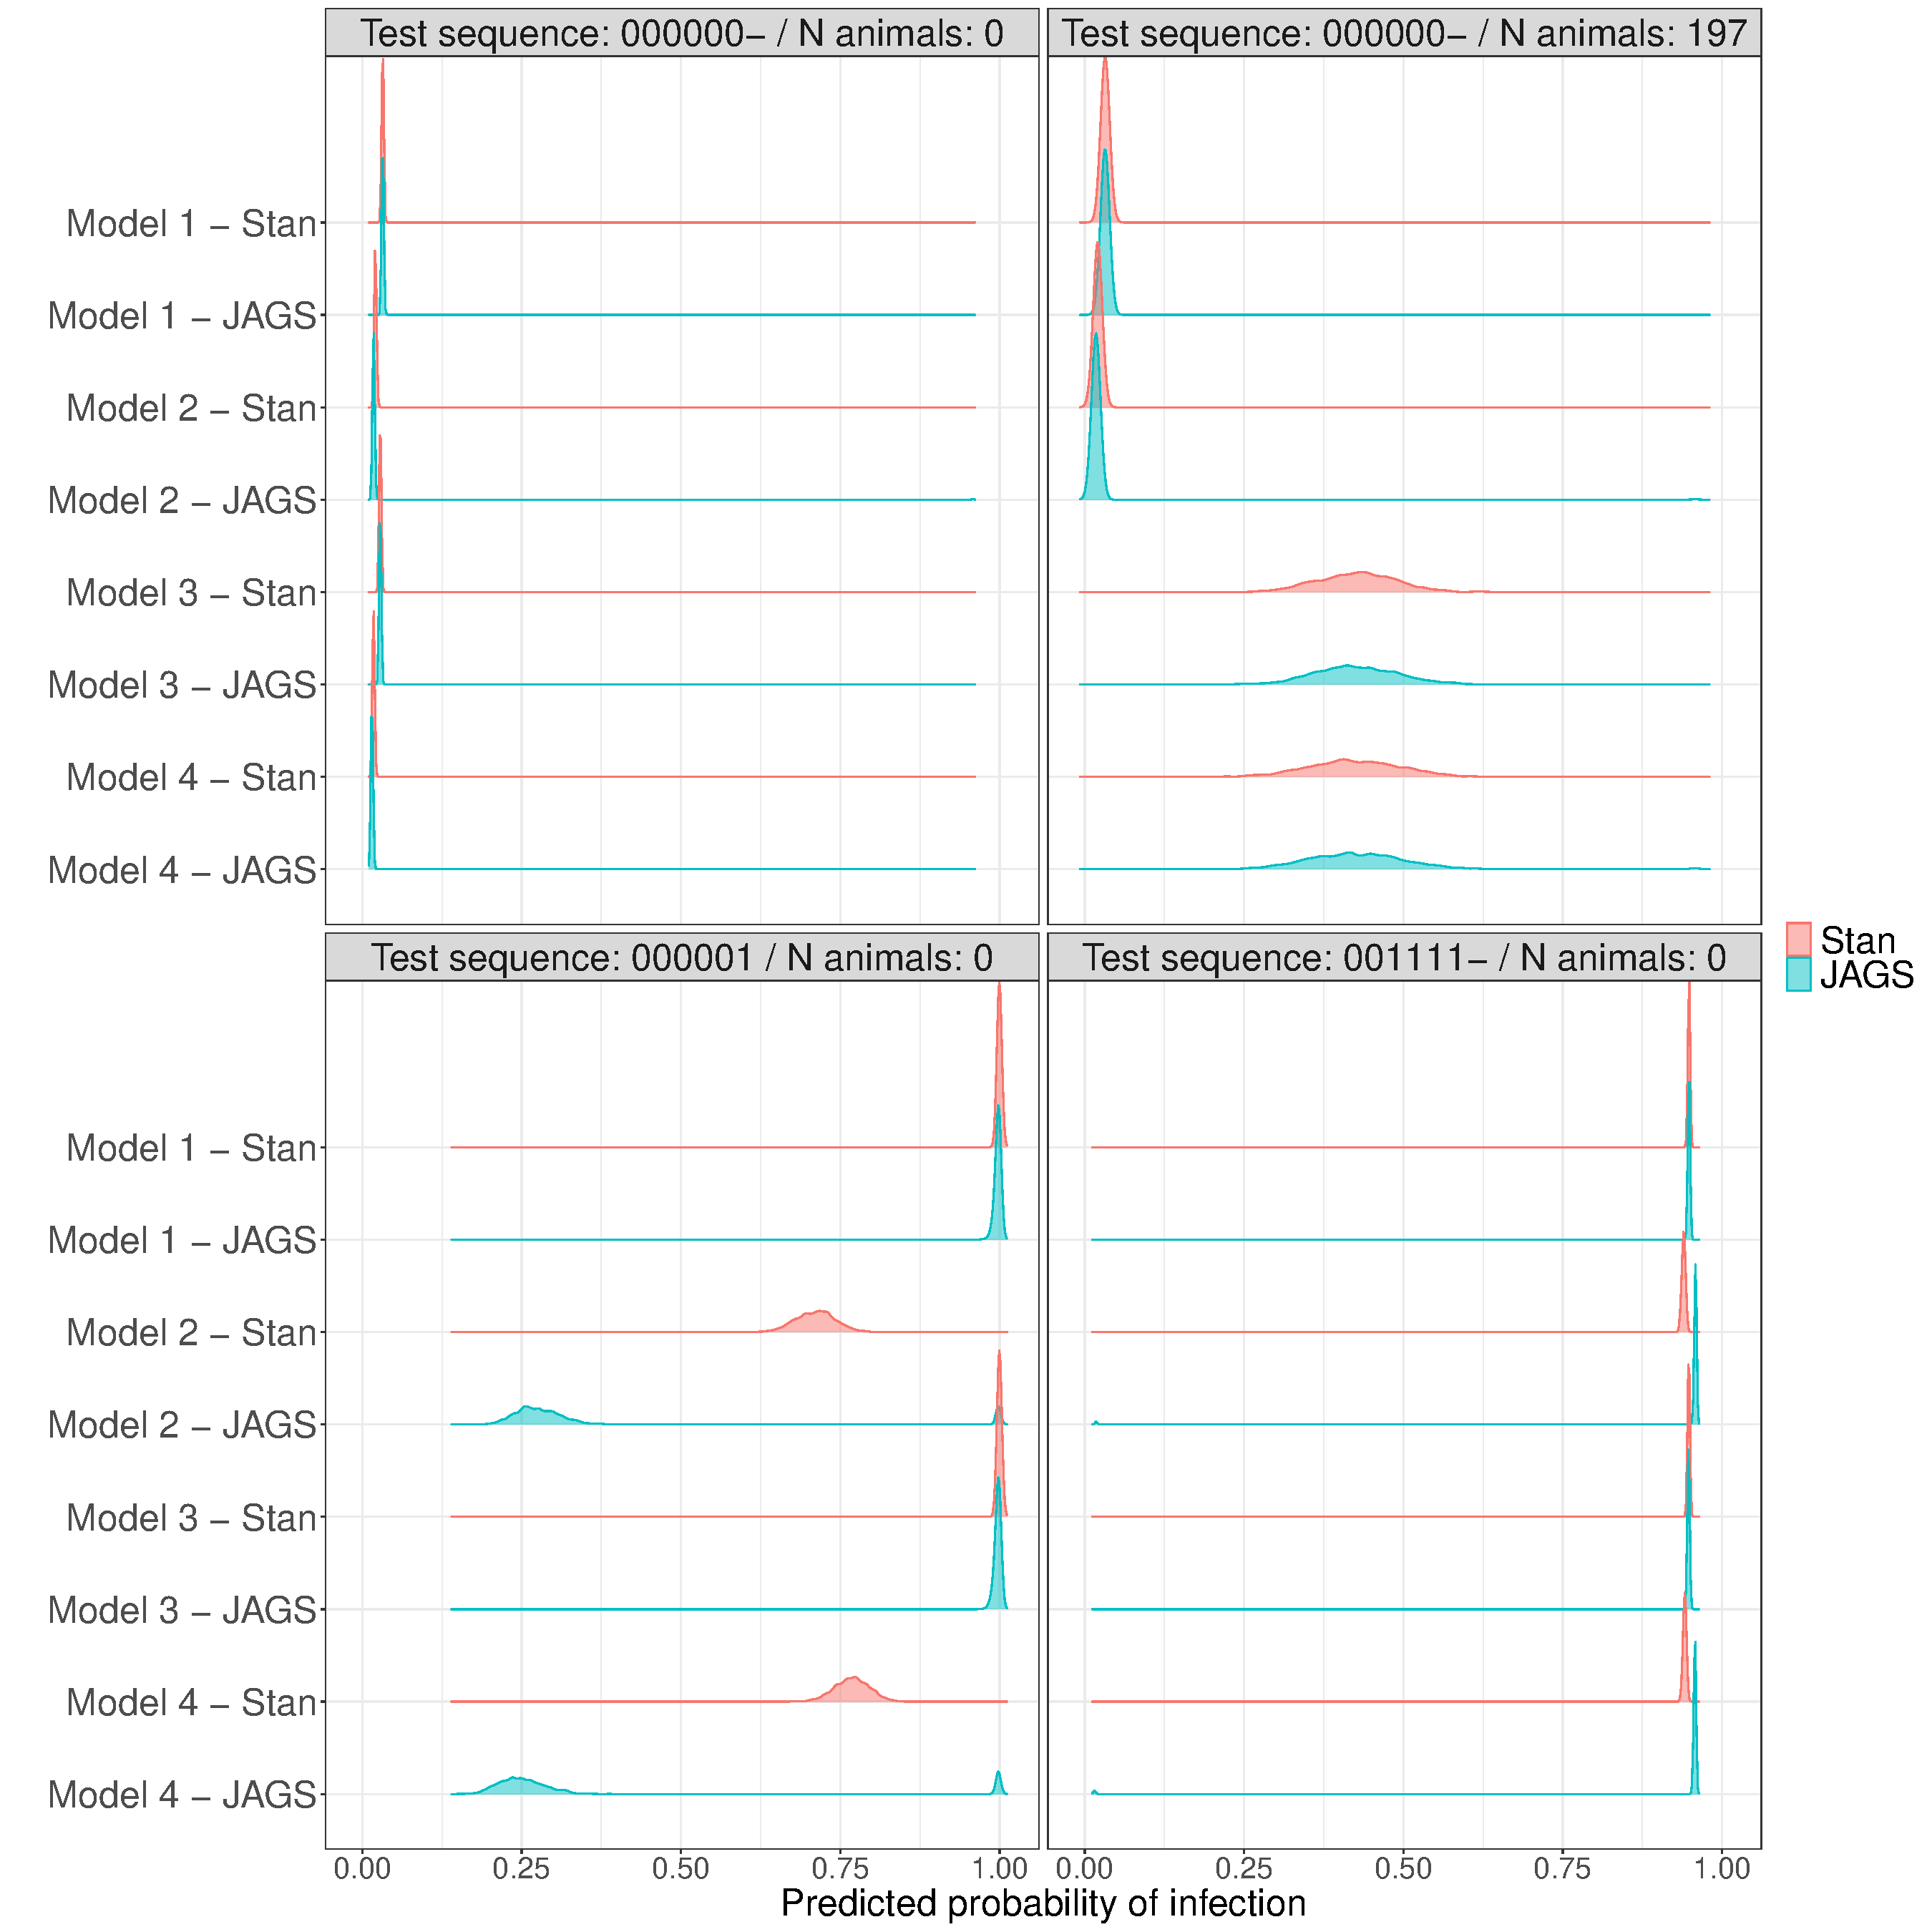
\includegraphics[width=.72\textwidth]{imgs/plot_predicted_proba_4herds.pdf}
\end{frame}

\begin{frame}
\frametitle{Take home}
 \begin{itemize}
  \item{The \texttt{STOC free} model predicts herd-level probabilities of infection from longitudinal surveillance data}
  \item<2->{Estimation / prediction in a Bayesian framework:}
  \begin{itemize}
   \item{allows the incorporation of available knowledge on test characteristics and disease epidemiology in a straightforward way using prior distributions}
   \item{the Stan implementation converges much better than the JAGS implementation}
  \end{itemize}
  \item<3->{Further work:}
  \begin{itemize}
   \item{Categorise herds into infection free / not free from the predicted posterior distributions of infection}
   \item{How to define prior distributions for herd-level test characteristics?}
  \end{itemize}
  \item<4->{All code and documentation available on Github}
  \begin{itemize}
   \item{R package, submitted paper, this presentation and a tutorial}
   \item[$\Rightarrow$]{please use and improve $\ldots$}
  \end{itemize}
 \end{itemize}
\end{frame}

\begin{frame}
\frametitle{Take home}
\begin{itemize}
  \item{All code and documentation available on Github}
  \begin{itemize}
   \item{R package: \url{https://github.com/AurMad/STOCfree}}
   \item{Submitted paper: \url{https://www.biorxiv.org/content/10.1101/2020.07.10.197426v4}}
   \item{This presentation and a tutorial: \url{https://github.com/AurMad/STOCfree_model_tutorial}}
  \end{itemize}
   \item[$\Rightarrow$]{please use and improve !}
 \end{itemize}
\end{frame}

{
    \usebackgroundtemplate{
\includegraphics[height=\paperheight,width=\paperwidth]{imgs/last_slide.png}}
    \setbeamertemplate{navigation symbols}{}
    \begin{frame}[plain]
    \end{frame}
    }

\end{document}
